\subsection{REAL-VALUED FUNCTIONS DEFINED ON A FILTERED SET}

PROPOSITION 1. Let \(f\) and \(g\) be two real-valued functions defined on a set \(\mathbf{X}\) filtered by a filter \(\mathfrak{F}\) . If \(\lim_{\mathfrak{F}} f\) and \(\lim_{\mathfrak{F}} g\) exist, and if, for each subset \(\mathbf{A} \in \mathfrak{F}\) , there exists \(x \in \mathbf{A}\) such that \(f(x) \leqslant g(x)\) , then we have \(\lim_{\mathfrak{F}} f \leqslant \lim_{\mathfrak{F}} g\) .

To prove this result we shall prove the following equivalent statement:

PROPOSITION 2. Let \(f\) and \(g\) be two real-valued functions defined on a set \(X\) filtered by a filter \(\mathfrak{F}\) . If \(\lim_{\mathfrak{F}} f\) and \(\lim_{\mathfrak{F}} g\) exist, and if \(\lim_{\mathfrak{F}} f > \lim_{\mathfrak{F}} g\) , then there is a set \(A \in \mathfrak{F}\) such that \(f(x) > g(x)\) for all \(x \in A\) .

Let \(a = \lim_{\mathfrak{F}} f\) , let \(b = \lim_{\mathfrak{F}} g\) and let \(c\) be such that \(b < c < a\) . The interval \(]c, +\infty]\) of \(\overline{\mathbf{R}}\) (resp. \([-\infty, c[)\) is a neighbourhood of \(a\) (resp. \(b\) ); hence there is a set \(M \in \mathfrak{F}\) (resp. a set \(N \in \mathfrak{F}\) ) such that \(f(x) > c\) for all \(x \in M\) {[}resp. \(g(x) < c\) for all \(x \in N\) {]}. The set \(A = M \cap N\) belongs to \(\mathfrak{F}\) , and we have \(f(x) > c > g(x)\) for all \(x \in A\) .

As a particular case of Proposition 1 we have the following theorem:

THEOREM 1 (Principle of extension of inequalities). Let \(f\) and \(g\) be two real-valued functions, defined on a set \(\mathbf{X}\) filtered by a filter \(\mathfrak{F}\) . If \(\lim_{\mathfrak{F}} f\) and \(\lim_{\mathfrak{F}} g\) exist, and if \(f \leqslant g\) , then \(\lim_{\mathfrak{F}} f \leqslant \lim_{\mathfrak{F}} g\) .

\pandocbounded{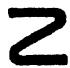
\includegraphics[keepaspectratio]{images/part002_67e89114.jpg}}

Remark. If in particular we have \(f(x) < g(x)\) for all \(x \in X\) (or only for all points of a set of the filter \(\overline{\mathbf{R}}\) ) we can infer, by Theorem 1, that \(\lim_{\mathfrak{F}} f \leqslant \lim_{\mathfrak{F}} g\) ; but we cannot infer the strong inequality \(\lim_{\mathfrak{F}} f < \lim_{\mathfrak{F}} g\) . For example, if we take \(X\) to be the set \(N\) of natural numbers, filtered by the Fréchet filter, and if \(f(n) = 0\) and \(g(n) = 1/n\) , then \(f(n) < g(n)\) for all \(n\) , but \(\lim_{n \to \infty} f(n) = \lim_{n \to \infty} f(n) = 0\) . Thus we lose strictness when we pass to the limit in a strict inequality.

THEOREM 2 (Theorem of the monotone limit). Let X be an ordered set and let A be a directed subset of X (*). Every monotonic real-valued function f defined on A has a limit with respect to A (Chapter I, § 7, no. 3); if f is increasing (resp. decreasing), this limit is equal to the least upper bound (resp. greatest lower bound) of the set \(f(A) \subset \overline{\mathbf{R}}\) .

Suppose for example that \(f\) is increasing, and let \(a = \sup f(A)\) . If \(a = -\infty\) , the theorem is trivial. If \(a > -\infty\) , then for each \(b < a\) there exists \(x \in A\) such that \(b < f(x) \leqslant a\) ; hence, if \(S_x\) is the section of \(A\) relative to \(x\) (i.e.~the set of all \(y \geqslant x\) , cf.~Chapter I, § 6, no. 3), \(f(S_x)\) is contained in the neighbourhood \(]b, +\infty]\) of \(a\) , and the theorem follows. The proof is analogous if \(f\) is decreasing.

COROLLARY. An increasing (resp. decreasing) real-valued function, defined on a directed subset A of an ordered set X, has a finite limit with respect to A if and only if it is bounded above (resp. bounded below) in A.

If we apply Theorem 2 to the case where \(\mathbf{A} = \mathbf{X} = \mathbf{N}\) (ordered by the relation \(\leqslant\) ), we have the following proposition:

PROPOSITION 3. Every monotonic sequence of real numbers has a limit in R. In particular, every increasing (resp. decreasing) sequence of finite numbers converges to a finite real number if it is bounded above (resp. bounded below) and to +∞ (resp. -∞) otherwise. For example, the sequence of positive integers converges to +∞.

This fact is the origin of the notation \(\lim_{n\to \infty}u_n\) to denote the limit of a sequence (Chapter I, § 7, no. 3).

Likewise, every strictly increasing sequence of integers \((p_n)\) converges to \(+\infty\) ; for we see by induction that \(p_n \geqslant p_0 + n\) for all \(n\) .

